Neste capítulo apresentamos o algoritmo \algname{Poset Forest Search} 
(\algname{PFS}), um algoritmo ótimo para o problema U-Curve que foi 
criado para enfrentar a limitação do algoritmo \algname{U-Curve Branch 
and Bound} (\algname{UBB}) ser unidirecional. Apesar do \algname{PFS}
ter solucionado tal problema com sucesso, este algoritmo apresenta 
pontos que ainda podem ser explorados para se criar uma modificação que
tenha melhor desempenho computacional. Modificaremos então o 
\algname{PFS}, explorando tais pontos.

\section{Descrição do algoritmo}
% - apresentar o UBB
%   - organização do espaço de busca em uma árvore
%   - pilha de busca em profundidade -> simples poda: não inserir nó
%     na pilha 
%   - limitação por ser unidirecional
% - apresentar o PFS
%   - duas florestas
%     - é bom explicar o que é leftmost aqui
%   - regras do jogo
%   - pseudo-código com as duas etapas
%   - indicar quais são os pontos que podem ser explorados

\subsection{O caso simples: \algname{U-Curve Branch and Bound}}
O algoritmo \algname{U-Curve Branch and Bound} (\algname{UBB}), que é 
uma versão simplificada do \algname{PFS}, percorre o espaço de busca 
fazendo uma busca em profundidade em uma árvore que é subgrafo do 
diagrama de Hasse do reticulado Booleano ($\powerset (S), \subseteq$). 
Esta árvore é definida por aplicações recursivas do seguinte lema:

\begin{mylemma}
\label{lemma:lower_forest}
Sejam $X$ e $Y$ conjunto, $X$ não-vazio e $I(i)$ o índice o $i$-ésimo 
elemento de $X$. Seja $X_0 \supseteq X_1 \supseteq \dots \supseteq 
X_{|X|}$ uma cadeia tal que $X_0 = X$, $X_{|X|} = \emptyset$ e $X_{i} 
\cup \{x_{I (i)}\} = X_{i - 1}$ para todo $0 < i \leq |X|$. Vale que:
\begin{align*}
\{ Y \} \cup \bigcup_{i = 1}^{|X|} \{W \cup Y \cup \{x_{I(i)}\} : W \in \powerset (X_i)\} = \{W \cup Y : W \in \powerset (X)\}.
\end{align*}
\end{mylemma} 

\begin{proof}
Faremos uma prova por indução no tamanho de $X$ de maneira similar a
Reis ~\cite{Rei12}.

\begin{itemize}
\item{Suponha que $|X| = 1$. Então:}
\begin{align*}
    \{Y\} \cup \bigcup_{i = 1}^{1} \{W \cup Y \cup \{x_i\} : W \in \powerset (X_i)\} & = 
    \{Y\} \cup \{W \cup Y \cup \{x_1\} : W \in \powerset (X_1)\} & \\
    & = \{Y\} \cup \{Y \cup \{x_1\}\} \tag{Como $X_1 = \emptyset$} \\
    & = \{Y, Y \cup \{x_1\}\} \\
    & = \{W \cup Y : W \in \powerset (X)\}
\end{align*}

\item{Suponha que o lema é verdadeiro para todo $X$ com $|X| < k$, 
    então:}
\begin{align*}
    & \{Y\} \cup \bigcup_{i = 1}^{k} \{W \cup Y \cup \{x_i\} : W \in \powerset (X_i)\} = \\
    & \{Y\} \cup \bigcup_{i = 2}^{k} \{W \cup Y \cup \{x_i\} : W \in \powerset (X_i)\} \cup \{W \cup Y \cup \{x_1\} : W \in \powerset (X_1) \}\\
\end{align*}
Seja $Z = Z_0 = X_1, Z_1 = X_2, \dots Z_{|Z|} = X_{|X|}$, então
$|Z| = k - 1$ e $z_1 = x_2, z_2 = x_3, \dots, z_{|Z|} = x_{|X|}$, e
\end{itemize}

\begin{align*}
    & \{Y\} \cup \bigcup_{i = 2}^{k} \{W \cup Y \cup \{x_i\} : W \in \powerset (X_i)\} \cup \{W \cup Y \cup \{x_1\} : W \in \powerset (X_1) \} =\\
    & \{Y\} \cup \bigcup_{j = 1}^{k - 1} \{W \cup Y \cup \{z_j\} : W \in \powerset (Z_i)\} \cup \{W \cup Y \cup \{x_1\} : W \in \powerset (X_1) \} =\\
    \tag{Pela hipótese de indução}  \\ 
    & \{Y \cup W : W \in \powerset (Z)\} \cup \{W \cup Y \cup \{x_1\} : W \in \powerset (X_1) \} =  \\
    & \{Y \cup W : W \in \powerset (X_1)\} \cup \{W \cup Y \cup \{x_1\} : W \in \powerset (X_1) \} =  \\
    & \{Y \cup W : W \in \powerset (X_1 \cup {x_1})\} = \\
    & \{Y \cup W : W \in \powerset (X)\} \\
\end{align*}
\end{proof}

Para representar o espaço de busca como uma árvore, devemos aplicar o
lema da seguinte forma. Vamos utilizar o conjunto $X_Y$ para determinar 
para cada nó $Y$ do reticulado quais são os nós alcançáveis por ele, de
maneira que um nó $Y$ pode alcançar todo nó do intervalo 
$[Y, X_Y \cup Y]$. Iniciamos a construção da árvore com a base da 
aplicação recursiva do lema, indicando que $X_{Y = \emptyset} = S$, 
pois $\emptyset$ deve ser a raiz da árvore e deve alcançar qualquer 
outro nó da árvore. Agora suponha que estamos em um nó $Y$, então
definimos $X_0 = X$, $X_{Y_i} \cup \{x_i\} = X_{Y_{i - 1}}$, e 
$Y_i = Y \cup \{x_i\}$ para $x_i \in X_Y$; então para criar a sub-árvore 
com raiz $Y$ basta adicionar os arcos $(Y, Y_i)$ para cada $i$ e aplicar 
o lema recursivamente para cada $Y_i$. A figura ~\ref{fig:pfs:ubb_tree} 
mostra uma árvore arbitrária gerada pela aplicação recursiva do lema 
~\ref{lemma:lower_forest}. 

\begin{figure}[!ht]
  \centering 
  \begin{tabular}{c c}
    \subfigure[] {\scalebox{0.4}{
     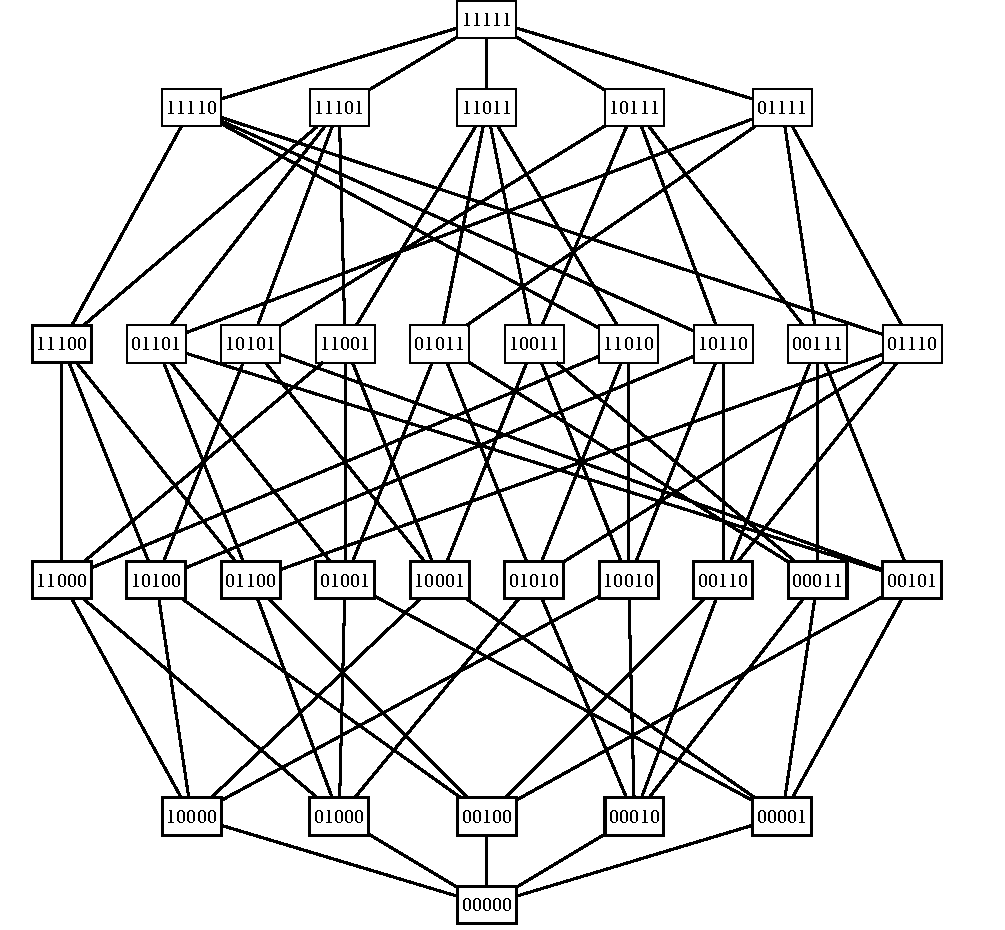
\includegraphics[clip=true]{pfs/ubb/full_lattice.pdf}}
     \label{fig:ubb:full} }
    & 
    \subfigure[] {\scalebox{.4}{
    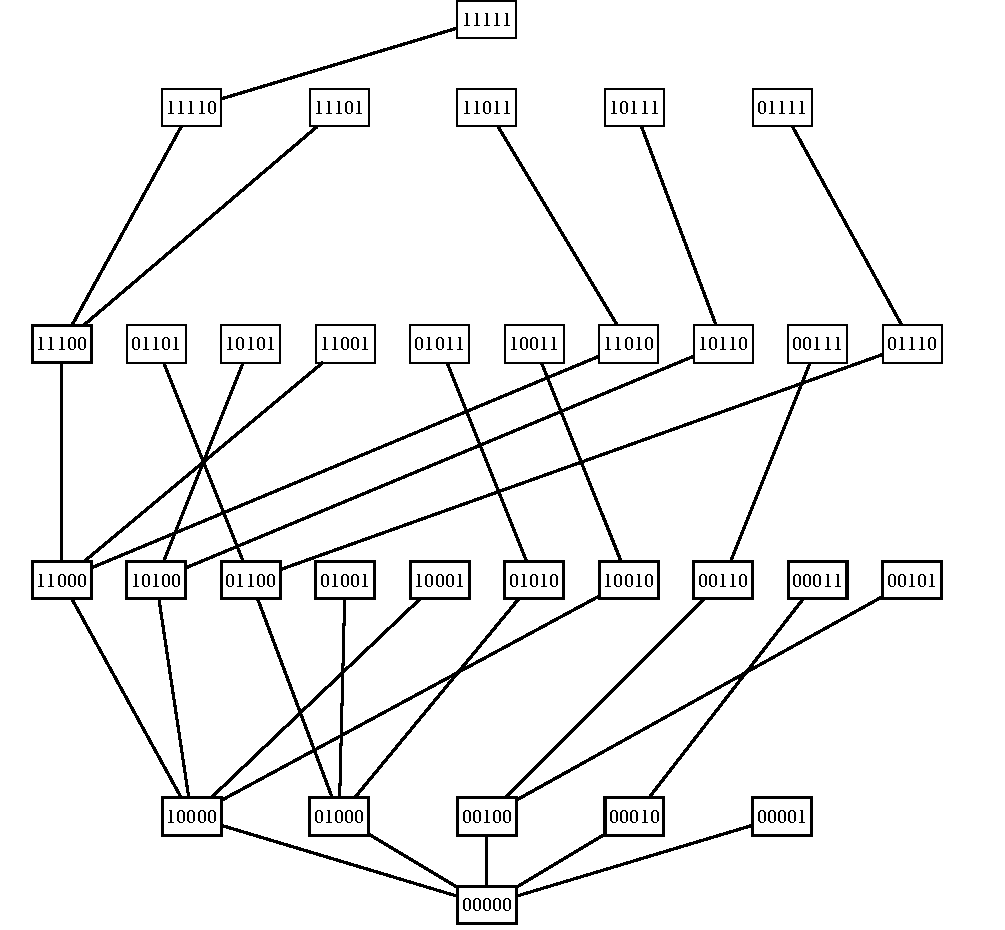
\includegraphics[clip=true]{pfs/ubb/ubb_tree.pdf}}
    \label{fig:ubb:tree} }
  \end{tabular}
    \caption{A figura ~\ref{fig:ubb:full} é o diagrama de Hasse do
    reticulado Booleano ($\powerset (S), \subseteq$) e a figura
    ~\ref{fig:ubb:tree} é uma árvore de busca definida pelo algoritmo
    \algname{UBB}.}
  \label{fig:pfs:ubb_tree} 
\end{figure}

A dinâmica deste algoritmo é simples. Aplica-se o lema 
~\ref{lemma:lower_forest} para percorrer o espaço de busca enquanto o 
custo dos subconjuntos se mantém ou diminui; quando o custo aumenta, 
podemos podar a sub-árvore que se inicia no nó onde o custo cresce. Por
exemplo, em uma instância do problema U-Curve com três características,
se o custo do nó $Y = \{100\}$ é maior do que o custo de $\{000\}$ e, ao 
visitar $Y$, $X = \{011\}$ então podemos remover do espaço de busca 
todos os nós do intervalo $[100, 111]$.


\begin{algorithm}[!ht]
\textsc{U-Curve-Branch-and-Bound} $(S, c)$
\begin{algorithmic}[1]
    \State $\mathcal{M} \gets \mathsc{Branch} (S, \emptyset, c, c (\emptyset))$
    \Return $\{M \in \mathcal{M} : c(M) \text{é mínimo}\}$
\end{algorithmic}
\vspace{1em}

\textsc{Branch} $(X, Y, c, cost_Y)$
\begin{algorithmic}[1]
    \State $\mathcal{M} \gets \{Y\}$
    \While{$X \ne \emptyset$}
        \State remova um elemento $x$ de $X$
        \State $Y' \gets Y \cup \{y\}$
        \State $cost_{Y'} \gets c (Y')$
        \If {$cost_{Y'} \leq cost_Y$}
            \State $\mathcal{N} \gets \mathsc{Branch} (X, Y', c, cost_{Y'})$
            \State $\mathcal{M} \gets \mathcal{N} \cup \mathcal{M}$
        \EndIf
    \EndWhile
    \Return $\mathcal{M}$
\end{algorithmic}
\caption{Pseudo-código do algoritmo \algname{UBB}}
\end{algorithm}

Uma vez entendido como as podas acontecem, é fácil perceber que o 
\algname{UBB} precisa percorrer uma cadeia inteira (não há podas) quando
o custo nela não aumenta até o penúltimo nó da cadeia. Portanto, se a 
função de custo é, por exemplo, monótona não-crescente, então a condição
de poda nunca será verdadeira em qualquer cadeia do reticulado, logo 
todo o espaço de busca será visitado, como em uma busca exaustiva. Esta
é a maior limitação do algoritmo \algname{UBB} e foi para enfrentá-la 
que o algoritmo \algname{PFS} foi criado.

\subsection{O algoritmo \algname{Poset-Forest-Search}}
% - criação das duas árvores
% - percorrimento e poda
% - como manter as duas árvores representando o mesmo espaço de busca?
%   - regras de poda
%   - florestas
% - 
O algoritmo \algname{Poset-Forest-Search} (\algname{PFS}) é uma 
generalização do \algname{UBB} capaz de percorrer o espaço de busca em
duas direções, do menor elemento do reticulado (como o \algname{UBB}) e
também do maior elemento para o menor. Para fazer isso, o \algname{PFS}
inicia sua busca com duas árvores complementares, uma gerada por 
aplicações recursivas do lema ~\ref{lemma:lower_forest} e outra, que 
representa o reticulado Booleano dual ($\powerset (S), \supseteq$), 
gerada por aplicações recursivas do lema ~\ref{lemma:upper_forest}.

\begin{mylemma}
\label{lemma:upper_forest}
Sejam $X$ e $Y$ conjunto, $X$ não-vazio e $I(i)$ o índice o $i$-ésimo 
elemento de $X$. Seja $X_0 \supseteq X_1 \supseteq \dots \supseteq 
X_{|X|}$ uma cadeia tal que $X_0 = X$, $X_{|X|} = \emptyset$ e $X_{i} 
\cup \{x_{I (i)}\} = X_{i - 1}$ para todo $0 < i \leq |X|$. Vale que:
\begin{align*}
    \{ Y \cup X\} \cup \bigcup_{i = 1}^{|X|} \{(X - (W \cup {x_{I(i)}})) \cup Y : W \in \powerset (X_i)\} = \{W \cup Y : W \in \powerset (X)\}.
\end{align*}
\end{mylemma} 

A figura ~\ref{fig:pfs:pfs_trees} mostra duas árvores do espaço de busca
geradas pelo algoritmo. Note que estas árvores permitem o percorrimento
do espaço de busca em duas direções.

\begin{figure}[!ht]
  \centering 
  \begin{tabular}{c c}
    \subfigure[] {\scalebox{0.4}{
     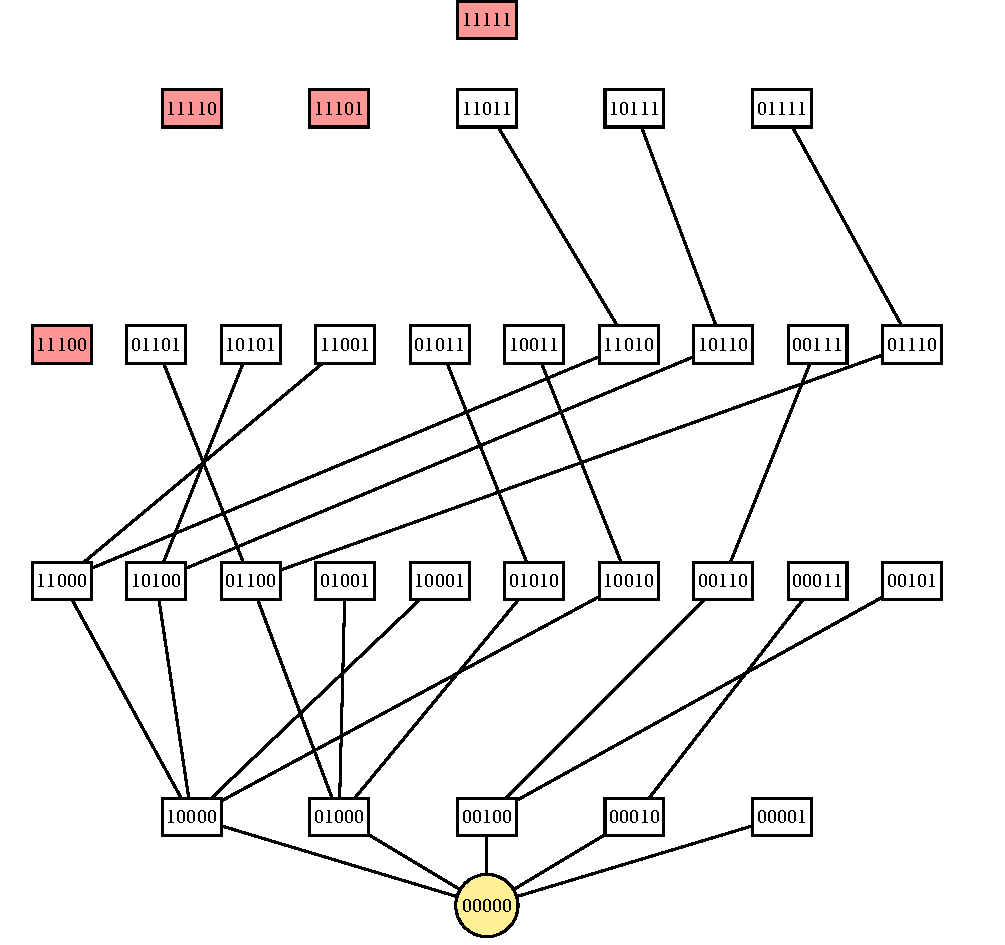
\includegraphics[clip=true]{pfs/pfs/lower_tree.pdf}}
     \label{fig:pfs:lower} }
    & 
    \subfigure[] {\scalebox{.4}{
    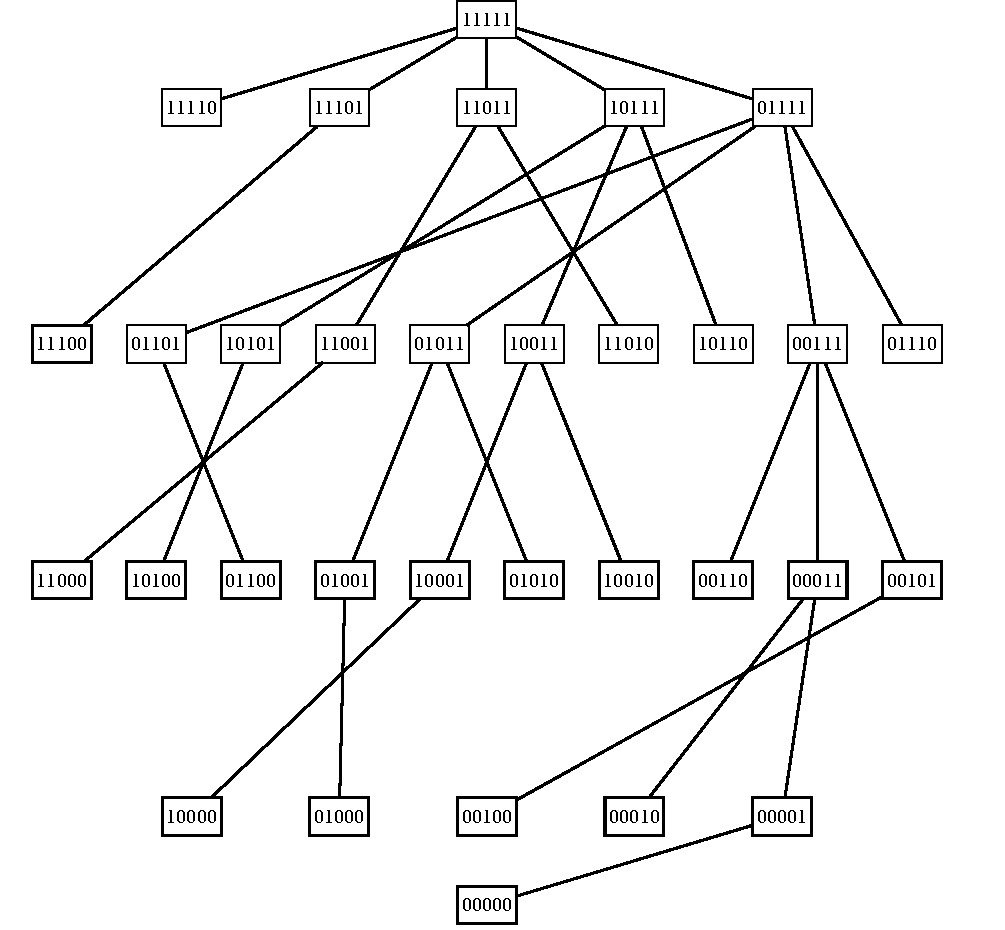
\includegraphics[clip=true]{pfs/pfs/upper_tree.pdf}}
    \label{fig:pfs:upper} }
  \end{tabular}
    \caption{Exemplo de árvores do espaço de busca gerado pelo 
    algoritmo \algname{PFS}. A figura ~\ref{fig:pfs:lower} mostra a 
    árvore gerada por aplicações recursivas do lema 
    ~\ref{lemma:lower_forest} enquanto a figura ~\ref{fig:pfs:upper} 
    mostra a árvore gerada por aplicações recursivas do lema 
    ~\ref{lemma:upper_forest}.}
  \label{fig:pfs:pfs_trees}
\end{figure}

No algoritmo \algname{UBB} o controle do espaço de busca pode ser 
facilmente implementado, pois basta não inserir a sub-árvore podada na 
pilha de busca em profundidade. No \algname{PFS}, uma estratégia 
equivalente é capaz apenas de restringir nós do espaço de busca que foi 
utilizado para o percorrimento de cadeias, ou seja, uma poda neste 
algoritmo implica na atualização das duas estruturas de dados que 
controlam o espaço de busca. 

\section{Melhoramentos na escolha de raiz}
% - aleatória
% - "leftmost"
\section{Melhoramentos no controle de raízes}
% - uso de ROBDD com as outras variações de raízes

\section{Paralelização do código}
